\section{Architecture}

The following picture shows the core components and interfaces

\begin{figure}[h]
    \centering
    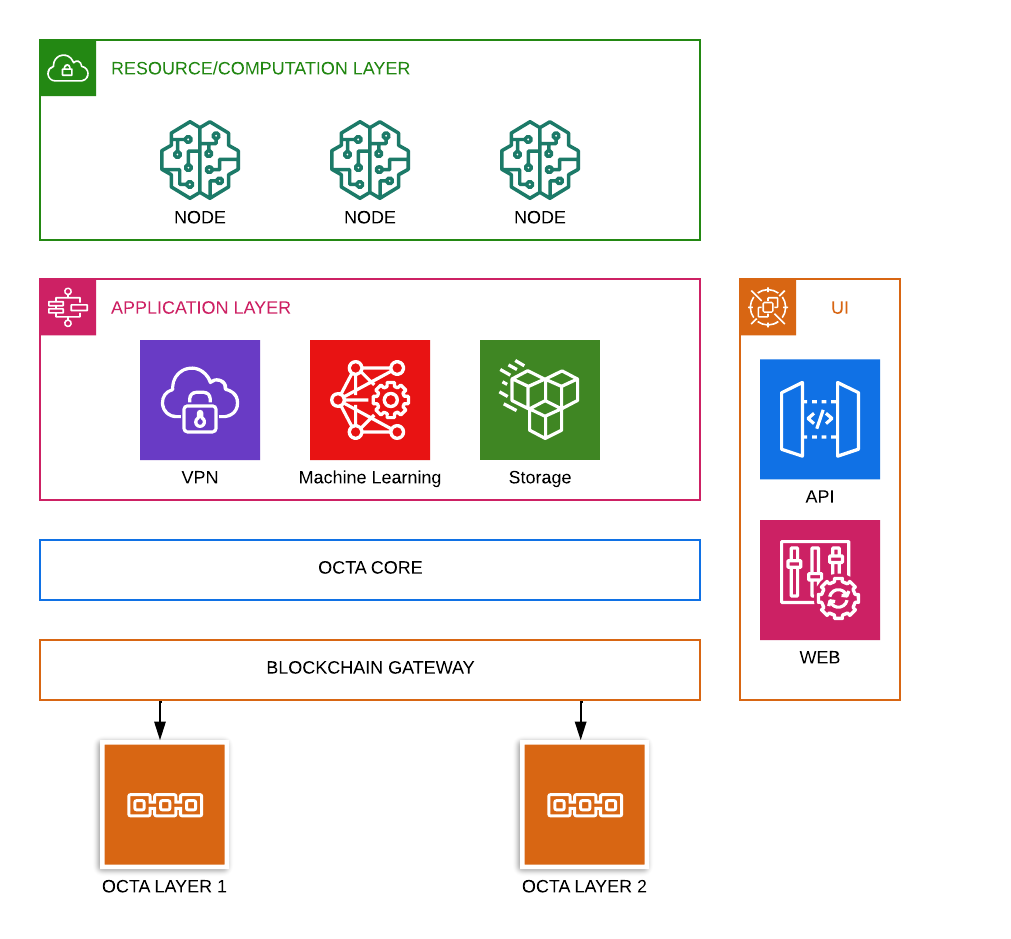
\includegraphics[width=\textwidth]{octa-arch}
    \caption{High Level Architecture}
\end{figure}

\subsection{Layer 1 network}

\textbf{OCTA Layer 1} is PoW\cite{pow} blockchain network is used for the frontend user financial operations using the native coin OCTA.

Network based on go-ethereum\cite{go-ethereum} codebase with the following specification:

\begin{itemize}
    \item Block time is 15 seconds
    \item Total supply is unlimited\footnote{Total supply will be reviewed after Mahasim fork}
    \item Block reward and halving implemented according to \hyperref[sec:mp]{Monenary policy}
    \item PirlGuard is used as protection mechanism from 51\% attack
    \item Transaction fee is 21 Gwei
\end{itemize}

Fair start of the network without premine and with genesis difficulty in 100Gh to prevent instant reward.

\subsection{Layer 2 network}

This is a side chain for Layer 1 network, implemented as PoA\cite{poa} network with a set of validators.

Used for handling internal transactions for the node services its lightning-fast performance and its seamlessly handling of high-frequency, high-usage operations,
resulting in reduced operational costs, speedy transactions and a massive boost in charging operations throughput.

\subsection{Blockchain gateways}

These gateways provides unified API for \textbf{OCTA CORE} layer to give it ability work with both blockchain networks.

This API is private and not accessible outside.

\subsection{OCTA CORE and Application Layer}

The core engine of our system, it's responsible for the following operations:

\begin{itemize}
    \item Communicates, monitoring and low level interaction with nodes
    \item Handle requests for computing resources
    \item Provide interface for creating services on a top of resources provided by nodes
    \item Services usage charging and billing operations
    \item Provide API for automation or integration with third party systems
    \item Fraud control
    \item Statistic and telemetry of system usage
\end{itemize}

\subsection{Resource Layer}

This layer consist of hardware(nodes) connected to the OctaSpace cloud.

Nodes are the foundation of our compute and services marketplace, providing the necessary computational power to meet the demands of tasks.

These computers are equipped with a blend of CPUs, GPUs, memory, and disk space that allows them to handle distributed workloads with ease.

The nodes are connected to the OctaSpace, which enables them to seamlessly work together to deliver optimal performance and efficiency.

The tasks and services may vary, well equipped machines with powerful GPU may performs AI/ML tasks,
common machines may acts as VPN gateway, provide disk storage for services like file sharing or host applications deployed by users.

In the nutshell node is a Linux machine with special software installed.

This software is called \textbf{ORC}, using it \textbf{OCTA CORE} is able to establish secure communication channel to the node.

Communication between \textbf{OCTA CORE} and \textbf{ORC} is doing in RPC\cite{rpc} like manner.

Secure channel is implemented using HTTPS\cite{https} protocol with validating each request using security token.

\begin{figure}[H]
    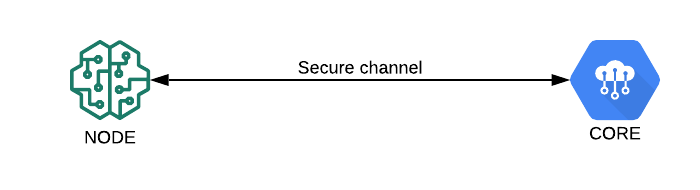
\includegraphics[width=\textwidth]{core-orc-channel}
    \caption{High Level Architecture}
\end{figure}

\subsection{API and UI}

To work with system the following interfaces available:

\begin{itemize}
    \item Web applicaton with user-friendly interface: \url{https://cube.octa.space}
    \item RESTful API
    \item \textbf{octactl} command-line utility that provide user friendly interface to RESTful API
\end{itemize}
